\documentclass[1p]{elsarticle_modified}
%\bibliographystyle{elsarticle-num}

%\usepackage[colorlinks]{hyperref}
%\usepackage{abbrmath_seonhwa} %\Abb, \Ascr, \Acal ,\Abf, \Afrak
\usepackage{amsfonts}
\usepackage{amssymb}
\usepackage{amsmath}
\usepackage{amsthm}
\usepackage{scalefnt}
\usepackage{amsbsy}
\usepackage{kotex}
\usepackage{caption}
\usepackage{subfig}
\usepackage{color}
\usepackage{graphicx}
\usepackage{xcolor} %% white, black, red, green, blue, cyan, magenta, yellow
\usepackage{float}
\usepackage{setspace}
\usepackage{hyperref}

\usepackage{tikz}
\usetikzlibrary{arrows}

\usepackage{multirow}
\usepackage{array} % fixed length table
\usepackage{hhline}

%%%%%%%%%%%%%%%%%%%%%
\makeatletter
\renewcommand*\env@matrix[1][\arraystretch]{%
	\edef\arraystretch{#1}%
	\hskip -\arraycolsep
	\let\@ifnextchar\new@ifnextchar
	\array{*\c@MaxMatrixCols c}}
\makeatother %https://tex.stackexchange.com/questions/14071/how-can-i-increase-the-line-spacing-in-a-matrix
%%%%%%%%%%%%%%%

\usepackage[normalem]{ulem}

\newcommand{\msout}[1]{\ifmmode\text{\sout{\ensuremath{#1}}}\else\sout{#1}\fi}
%SOURCE: \msout is \stkout macro in https://tex.stackexchange.com/questions/20609/strikeout-in-math-mode

\newcommand{\cancel}[1]{
	\ifmmode
	{\color{red}\msout{#1}}
	\else
	{\color{red}\sout{#1}}
	\fi
}

\newcommand{\add}[1]{
	{\color{blue}\uwave{#1}}
}

\newcommand{\replace}[2]{
	\ifmmode
	{\color{red}\msout{#1}}{\color{blue}\uwave{#2}}
	\else
	{\color{red}\sout{#1}}{\color{blue}\uwave{#2}}
	\fi
}

\newcommand{\Sol}{\mathcal{S}} %segment
\newcommand{\D}{D} %diagram
\newcommand{\A}{\mathcal{A}} %arc


%%%%%%%%%%%%%%%%%%%%%%%%%%%%%5 test

\def\sl{\operatorname{\textup{SL}}(2,\Cbb)}
\def\psl{\operatorname{\textup{PSL}}(2,\Cbb)}
\def\quan{\mkern 1mu \triangleright \mkern 1mu}

\theoremstyle{definition}
\newtheorem{thm}{Theorem}[section]
\newtheorem{prop}[thm]{Proposition}
\newtheorem{lem}[thm]{Lemma}
\newtheorem{ques}[thm]{Question}
\newtheorem{cor}[thm]{Corollary}
\newtheorem{defn}[thm]{Definition}
\newtheorem{exam}[thm]{Example}
\newtheorem{rmk}[thm]{Remark}
\newtheorem{alg}[thm]{Algorithm}

\newcommand{\I}{\sqrt{-1}}
\begin{document}

%\begin{frontmatter}
%
%\title{Boundary parabolic representations of knots up to 8 crossings}
%
%%% Group authors per affiliation:
%\author{Yunhi Cho} 
%\address{Department of Mathematics, University of Seoul, Seoul, Korea}
%\ead{yhcho@uos.ac.kr}
%
%
%\author{Seonhwa Kim} %\fnref{s_kim}}
%\address{Center for Geometry and Physics, Institute for Basic Science, Pohang, 37673, Korea}
%\ead{ryeona17@ibs.re.kr}
%
%\author{Hyuk Kim}
%\address{Department of Mathematical Sciences, Seoul National University, Seoul 08826, Korea}
%\ead{hyukkim@snu.ac.kr}
%
%\author{Seokbeom Yoon}
%\address{Department of Mathematical Sciences, Seoul National University, Seoul, 08826,  Korea}
%\ead{sbyoon15@snu.ac.kr}
%
%\begin{abstract}
%We find all boundary parabolic representation of knots up to 8 crossings.
%
%\end{abstract}
%\begin{keyword}
%    \MSC[2010] 57M25 
%\end{keyword}
%
%\end{frontmatter}

%\linenumbers
%\tableofcontents
%
\newcommand\colored[1]{\textcolor{white}{\rule[-0.35ex]{0.8em}{1.4ex}}\kern-0.8em\color{red} #1}%
%\newcommand\colored[1]{\textcolor{white}{ #1}\kern-2.17ex	\textcolor{white}{ #1}\kern-1.81ex	\textcolor{white}{ #1}\kern-2.15ex\color{red}#1	}

{\Large $\underline{11a_{352}~(K11a_{352})}$}

\setlength{\tabcolsep}{10pt}
\renewcommand{\arraystretch}{1.6}
\vspace{1cm}\begin{tabular}{m{100pt}>{\centering\arraybackslash}m{274pt}}
\multirow{5}{120pt}{
	\centering
	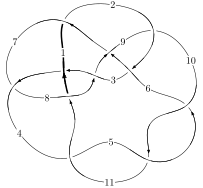
\includegraphics[width=112pt]{../../../GIT/diagram.site/Diagrams/png/601_11a_352.png}\\
\ \ \ A knot diagram\footnotemark}&
\allowdisplaybreaks
\textbf{Linearized knot diagam} \\
\cline{2-2}
 &
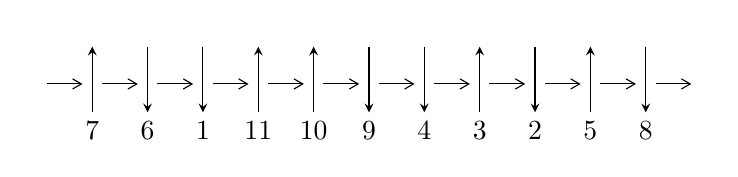
\begin{tikzpicture}[x=20pt, y=17pt]
	% nodes
	\node (C0) at (0, 0) {};
	\node (C1) at (1, 0) {};
	\node (C1U) at (1, +1) {};
	\node (C1D) at (1, -1) {7};

	\node (C2) at (2, 0) {};
	\node (C2U) at (2, +1) {};
	\node (C2D) at (2, -1) {6};

	\node (C3) at (3, 0) {};
	\node (C3U) at (3, +1) {};
	\node (C3D) at (3, -1) {1};

	\node (C4) at (4, 0) {};
	\node (C4U) at (4, +1) {};
	\node (C4D) at (4, -1) {11};

	\node (C5) at (5, 0) {};
	\node (C5U) at (5, +1) {};
	\node (C5D) at (5, -1) {10};

	\node (C6) at (6, 0) {};
	\node (C6U) at (6, +1) {};
	\node (C6D) at (6, -1) {9};

	\node (C7) at (7, 0) {};
	\node (C7U) at (7, +1) {};
	\node (C7D) at (7, -1) {4};

	\node (C8) at (8, 0) {};
	\node (C8U) at (8, +1) {};
	\node (C8D) at (8, -1) {3};

	\node (C9) at (9, 0) {};
	\node (C9U) at (9, +1) {};
	\node (C9D) at (9, -1) {2};

	\node (C10) at (10, 0) {};
	\node (C10U) at (10, +1) {};
	\node (C10D) at (10, -1) {5};

	\node (C11) at (11, 0) {};
	\node (C11U) at (11, +1) {};
	\node (C11D) at (11, -1) {8};
	\node (C12) at (12, 0) {};

	% arrows
	\draw[->,>={angle 60}]
	(C0) edge (C1) (C1) edge (C2) (C2) edge (C3) (C3) edge (C4) (C4) edge (C5) (C5) edge (C6) (C6) edge (C7) (C7) edge (C8) (C8) edge (C9) (C9) edge (C10) (C10) edge (C11) (C11) edge (C12) ;	\draw[->,>=stealth]
	(C1D) edge (C1U) (C2U) edge (C2D) (C3U) edge (C3D) (C4D) edge (C4U) (C5D) edge (C5U) (C6U) edge (C6D) (C7U) edge (C7D) (C8D) edge (C8U) (C9U) edge (C9D) (C10D) edge (C10U) (C11U) edge (C11D) ;
	\end{tikzpicture} \\
\hhline{~~} \\& 
\textbf{Solving Sequence} \\ \cline{2-2} 
 &
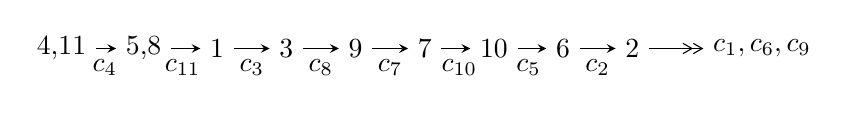
\begin{tikzpicture}[x=25pt, y=7pt]
	% node
	\node (A0) at (-1/8, 0) {4,11};
	\node (A1) at (17/16, 0) {5,8};
	\node (A2) at (17/8, 0) {1};
	\node (A3) at (25/8, 0) {3};
	\node (A4) at (33/8, 0) {9};
	\node (A5) at (41/8, 0) {7};
	\node (A6) at (49/8, 0) {10};
	\node (A7) at (57/8, 0) {6};
	\node (A8) at (65/8, 0) {2};
	\node (C1) at (1/2, -1) {$c_{4}$};
	\node (C2) at (13/8, -1) {$c_{11}$};
	\node (C3) at (21/8, -1) {$c_{3}$};
	\node (C4) at (29/8, -1) {$c_{8}$};
	\node (C5) at (37/8, -1) {$c_{7}$};
	\node (C6) at (45/8, -1) {$c_{10}$};
	\node (C7) at (53/8, -1) {$c_{5}$};
	\node (C8) at (61/8, -1) {$c_{2}$};
	\node (A9) at (10, 0) {$c_{1},c_{6},c_{9}$};

	% edge
	\draw[->,>=stealth]	
	(A0) edge (A1) (A1) edge (A2) (A2) edge (A3) (A3) edge (A4) (A4) edge (A5) (A5) edge (A6) (A6) edge (A7) (A7) edge (A8) ;
	\draw[->>,>={angle 60}]	
	(A8) edge (A9);
\end{tikzpicture} \\ 

\end{tabular} \\

\footnotetext{
The image of knot diagram is generated by the software ``\textbf{Draw programme}" developed by Andrew Bartholomew(\url{http://www.layer8.co.uk/maths/draw/index.htm\#Running-draw}), where we modified some parts for our purpose(\url{https://github.com/CATsTAILs/LinksPainter}).
}\phantom \\ \newline 
\centering \textbf{Ideals for irreducible components\footnotemark of $X_{\text{par}}$} 
 
\begin{align*}
I^u_{1}&=\langle 
-3 u^9+16 u^8-53 u^7+124 u^6-204 u^5+242 u^4-203 u^3+82 u^2+16 b+2 u-12,\\
\phantom{I^u_{1}}&\phantom{= \langle  }-3 u^9+24 u^8-101 u^7+292 u^6-620 u^5+978 u^4-1147 u^3+970 u^2+32 a-494 u+116,\\
\phantom{I^u_{1}}&\phantom{= \langle  }u^{10}-6 u^9+23 u^8-62 u^7+124 u^6-190 u^5+221 u^4-188 u^3+110 u^2-40 u+8\rangle \\
I^u_{2}&=\langle 
a u+b,\;-3 u^6 a+2 u^6+\cdots-12 a+17,\;u^7-4 u^6+11 u^5-20 u^4+26 u^3-23 u^2+14 u-4\rangle \\
I^u_{3}&=\langle 
-1348740987753 a^7 u^3+686668738913 a^6 u^3+\cdots-41120280504 a+141432788735,\\
\phantom{I^u_{3}}&\phantom{= \langle  }- a^7 u^3-4 a^6 u^3+\cdots+10 a+96,\;u^4+u^3+3 u^2+2 u+1\rangle \\
I^u_{4}&=\langle 
11 a^3 u^3+16 u^3 a^2+\cdots-5 a-3,\\
\phantom{I^u_{4}}&\phantom{= \langle  }a^3 u^3- u^3 a^2+a^4+2 a^3 u-2 u^3 a-2 a^2 u-3 u^2 a-2 u^3+a^2-5 a u-2 u^2-6 a-5 u-4,\\
\phantom{I^u_{4}}&\phantom{= \langle  }u^4+u^3+3 u^2+2 u+1\rangle \\
I^u_{5}&=\langle 
- u^{15}+u^{14}-11 u^{13}+9 u^{12}-46 u^{11}+30 u^{10}-87 u^9+44 u^8-63 u^7+24 u^6+u^5+u^4+3 u^2+2 b-9 u+3,\\
\phantom{I^u_{5}}&\phantom{= \langle  }-3 u^{15}-5 u^{14}+\cdots+10 a-45,\;u^{16}+11 u^{14}+47 u^{12}+96 u^{10}+90 u^8+26 u^6- u^4+8 u^2+5\rangle \\
I^u_{6}&=\langle 
- u^3- a u- u^2+b-2 u-1,\;- u^3 a- u^3+a^2-2 a u-2 u+1,\;u^4+u^3+3 u^2+2 u+1\rangle \\
I^u_{7}&=\langle 
u^3- u^2+b+2 u-1,\;- u^3+a-2 u,\;u^4- u^3+3 u^2-2 u+1\rangle \\
\\
I^v_{1}&=\langle 
a,\;b-1,\;v+1\rangle \\
\end{align*}
\raggedright * 8 irreducible components of $\dim_{\mathbb{C}}=0$, with total 101 representations.\\
\footnotetext{All coefficients of polynomials are rational numbers. But the coefficients are sometimes approximated in decimal forms when there is not enough margin.}
\newpage
\renewcommand{\arraystretch}{1}
\centering \section*{I. $I^u_{1}= \langle -3 u^9+16 u^8+\cdots+16 b-12,\;-3 u^9+24 u^8+\cdots+32 a+116,\;u^{10}-6 u^9+\cdots-40 u+8 \rangle$}
\flushleft \textbf{(i) Arc colorings}\\
\begin{tabular}{m{7pt} m{180pt} m{7pt} m{180pt} }
\flushright $a_{4}=$&$\begin{pmatrix}1\\0\end{pmatrix}$ \\
\flushright $a_{11}=$&$\begin{pmatrix}0\\u\end{pmatrix}$ \\
\flushright $a_{5}=$&$\begin{pmatrix}1\\- u^2\end{pmatrix}$ \\
\flushright $a_{8}=$&$\begin{pmatrix}\frac{3}{32} u^9-\frac{3}{4} u^8+\cdots+\frac{247}{16} u-\frac{29}{8}\\\frac{3}{16} u^9- u^8+\cdots-\frac{1}{8} u+\frac{3}{4}\end{pmatrix}$ \\
\flushright $a_{1}=$&$\begin{pmatrix}\frac{13}{32} u^9-2 u^8+\cdots+\frac{73}{16} u+\frac{1}{8}\\-\frac{7}{16} u^9+\frac{5}{2} u^8+\cdots-\frac{123}{8} u+\frac{13}{4}\end{pmatrix}$ \\
\flushright $a_{3}=$&$\begin{pmatrix}\frac{3}{32} u^9-\frac{3}{4} u^8+\cdots+\frac{167}{16} u-\frac{13}{8}\\\frac{5}{16} u^9-2 u^8+\cdots+\frac{105}{8} u-\frac{11}{4}\end{pmatrix}$ \\
\flushright $a_{9}=$&$\begin{pmatrix}\frac{3}{32} u^9-\frac{1}{2} u^8+\cdots+\frac{55}{16} u-\frac{1}{8}\\\frac{7}{16} u^9-\frac{3}{2} u^8+\cdots-\frac{5}{8} u+\frac{3}{4}\end{pmatrix}$ \\
\flushright $a_{7}=$&$\begin{pmatrix}\frac{9}{32} u^9-\frac{7}{4} u^8+\cdots+\frac{245}{16} u-\frac{23}{8}\\\frac{3}{16} u^9- u^8+\cdots-\frac{1}{8} u+\frac{3}{4}\end{pmatrix}$ \\
\flushright $a_{10}=$&$\begin{pmatrix}- u\\u^3+u\end{pmatrix}$ \\
\flushright $a_{6}=$&$\begin{pmatrix}u^2+1\\- u^4-2 u^2\end{pmatrix}$ \\
\flushright $a_{2}=$&$\begin{pmatrix}\frac{5}{32} u^9-\frac{3}{4} u^8+\cdots+\frac{113}{16} u-\frac{11}{8}\\-\frac{3}{16} u^9+u^8+\cdots+\frac{17}{8} u-\frac{3}{4}\end{pmatrix}$\\ \flushright $a_{2}=$&$\begin{pmatrix}\frac{5}{32} u^9-\frac{3}{4} u^8+\cdots+\frac{113}{16} u-\frac{11}{8}\\-\frac{3}{16} u^9+u^8+\cdots+\frac{17}{8} u-\frac{3}{4}\end{pmatrix}$\\&\end{tabular}
\flushleft \textbf{(ii) Obstruction class $= -1$}\\~\\
\flushleft \textbf{(iii) Cusp Shapes $= \frac{3}{4} u^9-3 u^8+\frac{45}{4} u^7-24 u^6+43 u^5-\frac{105}{2} u^4+\frac{187}{4} u^3-\frac{47}{2} u^2-\frac{9}{2} u+5$}\\~\\
\newpage\renewcommand{\arraystretch}{1}
\flushleft \textbf{(iv) u-Polynomials at the component}\newline \\
\begin{tabular}{m{50pt}|m{274pt}}
Crossings & \hspace{64pt}u-Polynomials at each crossing \\
\hline $$\begin{aligned}c_{1},c_{8}\end{aligned}$$&$\begin{aligned}
&u^{10}+u^9+7 u^8+4 u^7+23 u^6+9 u^5+40 u^4+9 u^3+33 u^2+2 u+10
\end{aligned}$\\
\hline $$\begin{aligned}c_{2},c_{7},c_{9}\\c_{11}\end{aligned}$$&$\begin{aligned}
&u^{10}+u^9- u^8-2 u^7+5 u^6+3 u^5-3 u^3- u+1
\end{aligned}$\\
\hline $$\begin{aligned}c_{3},c_{6}\end{aligned}$$&$\begin{aligned}
&u^{10}-9 u^9+\cdots-15 u+11
\end{aligned}$\\
\hline $$\begin{aligned}c_{4},c_{5},c_{10}\end{aligned}$$&$\begin{aligned}
&u^{10}-6 u^9+\cdots-40 u+8
\end{aligned}$\\
\hline
\end{tabular}\\~\\
\newpage\renewcommand{\arraystretch}{1}
\flushleft \textbf{(v) Riley Polynomials at the component}\newline \\
\begin{tabular}{m{50pt}|m{274pt}}
Crossings & \hspace{64pt}Riley Polynomials at each crossing \\
\hline $$\begin{aligned}c_{1},c_{8}\end{aligned}$$&$\begin{aligned}
&y^{10}+13 y^9+\cdots+656 y+100
\end{aligned}$\\
\hline $$\begin{aligned}c_{2},c_{7},c_{9}\\c_{11}\end{aligned}$$&$\begin{aligned}
&y^{10}-3 y^9+15 y^8-20 y^7+43 y^6-17 y^5+12 y^4+7 y^3-6 y^2- y+1
\end{aligned}$\\
\hline $$\begin{aligned}c_{3},c_{6}\end{aligned}$$&$\begin{aligned}
&y^{10}+3 y^9+\cdots+1601 y+121
\end{aligned}$\\
\hline $$\begin{aligned}c_{4},c_{5},c_{10}\end{aligned}$$&$\begin{aligned}
&y^{10}+10 y^9+\cdots+160 y+64
\end{aligned}$\\
\hline
\end{tabular}\\~\\
\newpage\flushleft \textbf{(vi) Complex Volumes and Cusp Shapes}
$$\begin{array}{c|c|c}  
\text{Solutions to }I^u_{1}& \I (\text{vol} + \sqrt{-1}CS) & \text{Cusp shape}\\
 \hline 
\begin{aligned}
u &= \phantom{-}0.827139 + 0.827690 I \\
a &= \phantom{-}0.124534 - 1.186260 I \\
b &= -1.084860 + 0.878124 I\end{aligned}
 & -3.86930 + 13.03600 I & -4.42534 - 9.74427 I \\ \hline\begin{aligned}
u &= \phantom{-}0.827139 - 0.827690 I \\
a &= \phantom{-}0.124534 + 1.186260 I \\
b &= -1.084860 - 0.878124 I\end{aligned}
 & -3.86930 - 13.03600 I & -4.42534 + 9.74427 I \\ \hline\begin{aligned}
u &= \phantom{-}1.231820 + 0.302946 I \\
a &= -0.687720 - 0.315351 I \\
b &= \phantom{-}0.751611 + 0.596797 I\end{aligned}
 & -2.14694 - 6.57736 I & -5.40678 + 10.73292 I \\ \hline\begin{aligned}
u &= \phantom{-}1.231820 - 0.302946 I \\
a &= -0.687720 + 0.315351 I \\
b &= \phantom{-}0.751611 - 0.596797 I\end{aligned}
 & -2.14694 + 6.57736 I & -5.40678 - 10.73292 I \\ \hline\begin{aligned}
u &= \phantom{-}0.314386 + 0.484120 I \\
a &= \phantom{-}0.850851 + 0.785005 I \\
b &= \phantom{-}0.112541 - 0.658708 I\end{aligned}
 & \phantom{-}0.232399 + 1.335330 I & \phantom{-}1.84390 - 5.86434 I \\ \hline\begin{aligned}
u &= \phantom{-}0.314386 - 0.484120 I \\
a &= \phantom{-}0.850851 - 0.785005 I \\
b &= \phantom{-}0.112541 + 0.658708 I\end{aligned}
 & \phantom{-}0.232399 - 1.335330 I & \phantom{-}1.84390 + 5.86434 I \\ \hline\begin{aligned}
u &= \phantom{-}0.25828 + 1.65152 I \\
a &= \phantom{-}0.458885 + 0.901810 I \\
b &= \phantom{-}1.37084 - 0.99078 I\end{aligned}
 & -12.0871 + 17.1582 I & -6.40595 - 8.48495 I \\ \hline\begin{aligned}
u &= \phantom{-}0.25828 - 1.65152 I \\
a &= \phantom{-}0.458885 - 0.901810 I \\
b &= \phantom{-}1.37084 + 0.99078 I\end{aligned}
 & -12.0871 - 17.1582 I & -6.40595 + 8.48495 I \\ \hline\begin{aligned}
u &= \phantom{-}0.36838 + 1.94011 I \\
a &= \phantom{-}0.003450 - 0.334444 I \\
b &= -0.650130 + 0.116508 I\end{aligned}
 & -9.27048 + 0.95500 I & -15.6058 - 6.9472 I \\ \hline\begin{aligned}
u &= \phantom{-}0.36838 - 1.94011 I \\
a &= \phantom{-}0.003450 + 0.334444 I \\
b &= -0.650130 - 0.116508 I\end{aligned}
 & -9.27048 - 0.95500 I & -15.6058 + 6.9472 I\\
 \hline 
 \end{array}$$\newpage\newpage\renewcommand{\arraystretch}{1}
\centering \section*{II. $I^u_{2}= \langle a u+b,\;-3 u^6 a+2 u^6+\cdots-12 a+17,\;u^7-4 u^6+\cdots+14 u-4 \rangle$}
\flushleft \textbf{(i) Arc colorings}\\
\begin{tabular}{m{7pt} m{180pt} m{7pt} m{180pt} }
\flushright $a_{4}=$&$\begin{pmatrix}1\\0\end{pmatrix}$ \\
\flushright $a_{11}=$&$\begin{pmatrix}0\\u\end{pmatrix}$ \\
\flushright $a_{5}=$&$\begin{pmatrix}1\\- u^2\end{pmatrix}$ \\
\flushright $a_{8}=$&$\begin{pmatrix}a\\- a u\end{pmatrix}$ \\
\flushright $a_{1}=$&$\begin{pmatrix}-\frac{1}{2} u^6 a+\frac{1}{4} u^6+\cdots-3 a+2\\-\frac{1}{2} u^6+u^5+\cdots+2 a-1\end{pmatrix}$ \\
\flushright $a_{3}=$&$\begin{pmatrix}-\frac{1}{4} u^6+\frac{1}{2} u^5+\cdots- a-1\\- u^5 a+\frac{3}{2} u^6+\cdots-\frac{15}{2} u+3\end{pmatrix}$ \\
\flushright $a_{9}=$&$\begin{pmatrix}\frac{1}{2} u^6 a-\frac{1}{4} u^6+\cdots+a-\frac{3}{2}\\- u^6 a+3 u^5 a+\cdots-2 a-1\end{pmatrix}$ \\
\flushright $a_{7}=$&$\begin{pmatrix}- a u+a\\- a u\end{pmatrix}$ \\
\flushright $a_{10}=$&$\begin{pmatrix}- u\\u^3+u\end{pmatrix}$ \\
\flushright $a_{6}=$&$\begin{pmatrix}u^2+1\\- u^4-2 u^2\end{pmatrix}$ \\
\flushright $a_{2}=$&$\begin{pmatrix}\frac{1}{4} u^6-\frac{1}{2} u^5+\cdots- a+2\\-\frac{1}{2} u^6+u^5+\cdots+\frac{5}{2} u-1\end{pmatrix}$\\ \flushright $a_{2}=$&$\begin{pmatrix}\frac{1}{4} u^6-\frac{1}{2} u^5+\cdots- a+2\\-\frac{1}{2} u^6+u^5+\cdots+\frac{5}{2} u-1\end{pmatrix}$\\&\end{tabular}
\flushleft \textbf{(ii) Obstruction class $= -1$}\\~\\
\flushleft \textbf{(iii) Cusp Shapes $= 5 u^6-13 u^5+32 u^4-44 u^3+46 u^2-32 u+14$}\\~\\
\newpage\renewcommand{\arraystretch}{1}
\flushleft \textbf{(iv) u-Polynomials at the component}\newline \\
\begin{tabular}{m{50pt}|m{274pt}}
Crossings & \hspace{64pt}u-Polynomials at each crossing \\
\hline $$\begin{aligned}c_{1},c_{8}\end{aligned}$$&$\begin{aligned}
&(u^7+u^5+u^4- u-1)^2
\end{aligned}$\\
\hline $$\begin{aligned}c_{2},c_{7},c_{9}\\c_{11}\end{aligned}$$&$\begin{aligned}
&u^{14}+u^{13}+\cdots+u+1
\end{aligned}$\\
\hline $$\begin{aligned}c_{3},c_{6}\end{aligned}$$&$\begin{aligned}
&u^{14}-13 u^{13}+\cdots-329 u+47
\end{aligned}$\\
\hline $$\begin{aligned}c_{4},c_{5},c_{10}\end{aligned}$$&$\begin{aligned}
&(u^7-4 u^6+11 u^5-20 u^4+26 u^3-23 u^2+14 u-4)^2
\end{aligned}$\\
\hline
\end{tabular}\\~\\
\newpage\renewcommand{\arraystretch}{1}
\flushleft \textbf{(v) Riley Polynomials at the component}\newline \\
\begin{tabular}{m{50pt}|m{274pt}}
Crossings & \hspace{64pt}Riley Polynomials at each crossing \\
\hline $$\begin{aligned}c_{1},c_{8}\end{aligned}$$&$\begin{aligned}
&(y^7+2 y^6+y^5-3 y^4-2 y^3+2 y^2+y-1)^2
\end{aligned}$\\
\hline $$\begin{aligned}c_{2},c_{7},c_{9}\\c_{11}\end{aligned}$$&$\begin{aligned}
&y^{14}-5 y^{13}+\cdots+y+1
\end{aligned}$\\
\hline $$\begin{aligned}c_{3},c_{6}\end{aligned}$$&$\begin{aligned}
&y^{14}-3 y^{13}+\cdots+2397 y+2209
\end{aligned}$\\
\hline $$\begin{aligned}c_{4},c_{5},c_{10}\end{aligned}$$&$\begin{aligned}
&(y^7+6 y^6+13 y^5+16 y^4+32 y^3+39 y^2+12 y-16)^2
\end{aligned}$\\
\hline
\end{tabular}\\~\\
\newpage\flushleft \textbf{(vi) Complex Volumes and Cusp Shapes}
$$\begin{array}{c|c|c}  
\text{Solutions to }I^u_{2}& \I (\text{vol} + \sqrt{-1}CS) & \text{Cusp shape}\\
 \hline 
\begin{aligned}
u &= \phantom{-}0.316075 + 1.084870 I \\
a &= \phantom{-}0.447890 + 1.041020 I \\
b &= \phantom{-}0.987810 - 0.814945 I\end{aligned}
 & -0.56973 + 3.46571 I & \phantom{-}1.80998 - 1.90405 I \\ \hline\begin{aligned}
u &= \phantom{-}0.316075 + 1.084870 I \\
a &= -0.468498 + 0.032326 I \\
b &= \phantom{-}0.183150 + 0.498043 I\end{aligned}
 & -0.56973 + 3.46571 I & \phantom{-}1.80998 - 1.90405 I \\ \hline\begin{aligned}
u &= \phantom{-}0.316075 - 1.084870 I \\
a &= \phantom{-}0.447890 - 1.041020 I \\
b &= \phantom{-}0.987810 + 0.814945 I\end{aligned}
 & -0.56973 - 3.46571 I & \phantom{-}1.80998 + 1.90405 I \\ \hline\begin{aligned}
u &= \phantom{-}0.316075 - 1.084870 I \\
a &= -0.468498 - 0.032326 I \\
b &= \phantom{-}0.183150 - 0.498043 I\end{aligned}
 & -0.56973 - 3.46571 I & \phantom{-}1.80998 + 1.90405 I \\ \hline\begin{aligned}
u &= \phantom{-}1.051270 + 0.735259 I \\
a &= -0.268053 + 0.911867 I \\
b &= \phantom{-}0.952255 - 0.761533 I\end{aligned}
 & -3.76584 + 3.52764 I & -10.39771 - 1.47160 I \\ \hline\begin{aligned}
u &= \phantom{-}1.051270 + 0.735259 I \\
a &= \phantom{-}0.591875 - 0.190941 I \\
b &= -0.762614 - 0.234450 I\end{aligned}
 & -3.76584 + 3.52764 I & -10.39771 - 1.47160 I \\ \hline\begin{aligned}
u &= \phantom{-}1.051270 - 0.735259 I \\
a &= -0.268053 - 0.911867 I \\
b &= \phantom{-}0.952255 + 0.761533 I\end{aligned}
 & -3.76584 - 3.52764 I & -10.39771 + 1.47160 I \\ \hline\begin{aligned}
u &= \phantom{-}1.051270 - 0.735259 I \\
a &= \phantom{-}0.591875 + 0.190941 I \\
b &= -0.762614 + 0.234450 I\end{aligned}
 & -3.76584 - 3.52764 I & -10.39771 + 1.47160 I \\ \hline\begin{aligned}
u &= \phantom{-}0.658991\phantom{ +0.000000I} \\
a &= \phantom{-}0.825920 + 1.123020 I \\
b &= -0.544274 - 0.740063 I\end{aligned}
 & \phantom{-}2.67359\phantom{ +0.000000I} & \phantom{-}5.12550\phantom{ +0.000000I} \\ \hline\begin{aligned}
u &= \phantom{-}0.658991\phantom{ +0.000000I} \\
a &= \phantom{-}0.825920 - 1.123020 I \\
b &= -0.544274 + 0.740063 I\end{aligned}
 & \phantom{-}2.67359\phantom{ +0.000000I} & \phantom{-}5.12550\phantom{ +0.000000I}\\
 \hline 
 \end{array}$$\newpage$$\begin{array}{c|c|c}  
\text{Solutions to }I^u_{2}& \I (\text{vol} + \sqrt{-1}CS) & \text{Cusp shape}\\
 \hline 
\begin{aligned}
u &= \phantom{-}0.30316 + 1.67229 I \\
a &= -0.402520 - 0.858604 I \\
b &= -1.31381 + 0.93342 I\end{aligned}
 & -11.8056 + 8.5528 I & -9.47503 - 5.91683 I \\ \hline\begin{aligned}
u &= \phantom{-}0.30316 + 1.67229 I \\
a &= \phantom{-}0.023386 + 0.600716 I \\
b &= \phantom{-}0.997484 - 0.221219 I\end{aligned}
 & -11.8056 + 8.5528 I & -9.47503 - 5.91683 I \\ \hline\begin{aligned}
u &= \phantom{-}0.30316 - 1.67229 I \\
a &= -0.402520 + 0.858604 I \\
b &= -1.31381 - 0.93342 I\end{aligned}
 & -11.8056 - 8.5528 I & -9.47503 + 5.91683 I \\ \hline\begin{aligned}
u &= \phantom{-}0.30316 - 1.67229 I \\
a &= \phantom{-}0.023386 - 0.600716 I \\
b &= \phantom{-}0.997484 + 0.221219 I\end{aligned}
 & -11.8056 - 8.5528 I & -9.47503 + 5.91683 I\\
 \hline 
 \end{array}$$\newpage\newpage\renewcommand{\arraystretch}{1}
\centering \section*{III. $I^u_{3}= \langle -1.35\times10^{12} a^{7} u^{3}+6.87\times10^{11} a^{6} u^{3}+\cdots-4.11\times10^{10} a+1.41\times10^{11},\;- a^7 u^3-4 a^6 u^3+\cdots+10 a+96,\;u^4+u^3+3 u^2+2 u+1 \rangle$}
\flushleft \textbf{(i) Arc colorings}\\
\begin{tabular}{m{7pt} m{180pt} m{7pt} m{180pt} }
\flushright $a_{4}=$&$\begin{pmatrix}1\\0\end{pmatrix}$ \\
\flushright $a_{11}=$&$\begin{pmatrix}0\\u\end{pmatrix}$ \\
\flushright $a_{5}=$&$\begin{pmatrix}1\\- u^2\end{pmatrix}$ \\
\flushright $a_{8}=$&$\begin{pmatrix}a\\2.06795 a^{7} u^{3}-1.05283 a^{6} u^{3}+\cdots+0.0630474 a-0.216851\end{pmatrix}$ \\
\flushright $a_{1}=$&$\begin{pmatrix}- a^2 u\\0.566545 a^{7} u^{3}-0.144764 a^{6} u^{3}+\cdots+0.0887731 a+1.58851\end{pmatrix}$ \\
\flushright $a_{3}=$&$\begin{pmatrix}0.0804851 a^{7} u^{3}+0.514618 a^{6} u^{3}+\cdots-1.21468 a+1.08057\\0.476938 a^{7} u^{3}+1.22479 a^{6} u^{3}+\cdots+0.337460 a+1.73643\end{pmatrix}$ \\
\flushright $a_{9}=$&$\begin{pmatrix}0.353631 a^{7} u^{3}-0.0766819 a^{6} u^{3}+\cdots-1.06770 a-1.03933\\0.277128 a^{7} u^{3}+0.0000142253 a^{6} u^{3}+\cdots-0.621680 a+0.912067\end{pmatrix}$ \\
\flushright $a_{7}=$&$\begin{pmatrix}2.06795 a^{7} u^{3}-1.05283 a^{6} u^{3}+\cdots+1.06305 a-0.216851\\2.06795 a^{7} u^{3}-1.05283 a^{6} u^{3}+\cdots+0.0630474 a-0.216851\end{pmatrix}$ \\
\flushright $a_{10}=$&$\begin{pmatrix}- u\\u^3+u\end{pmatrix}$ \\
\flushright $a_{6}=$&$\begin{pmatrix}u^2+1\\u^3+u^2+2 u+1\end{pmatrix}$ \\
\flushright $a_{2}=$&$\begin{pmatrix}1.50926 a^{7} u^{3}+1.35905 a^{6} u^{3}+\cdots-0.618723 a+0.472347\\2.16896 a^{7} u^{3}+0.686316 a^{6} u^{3}+\cdots+0.397134 a+1.30453\end{pmatrix}$\\ \flushright $a_{2}=$&$\begin{pmatrix}1.50926 a^{7} u^{3}+1.35905 a^{6} u^{3}+\cdots-0.618723 a+0.472347\\2.16896 a^{7} u^{3}+0.686316 a^{6} u^{3}+\cdots+0.397134 a+1.30453\end{pmatrix}$\\&\end{tabular}
\flushleft \textbf{(ii) Obstruction class $= -1$}\\~\\
\flushleft \textbf{(iii) Cusp Shapes $= -\frac{1367231366824}{326106026089} a^7 u^3-\frac{1370870830584}{326106026089} a^6 u^3+\cdots-\frac{3308821571992}{326106026089} a-\frac{4028263148378}{326106026089}$}\\~\\
\newpage\renewcommand{\arraystretch}{1}
\flushleft \textbf{(iv) u-Polynomials at the component}\newline \\
\begin{tabular}{m{50pt}|m{274pt}}
Crossings & \hspace{64pt}u-Polynomials at each crossing \\
\hline $$\begin{aligned}c_{1},c_{8}\end{aligned}$$&$\begin{aligned}
&(u^{16}- u^{15}+\cdots-24 u+79)^{2}
\end{aligned}$\\
\hline $$\begin{aligned}c_{2},c_{7},c_{9}\\c_{11}\end{aligned}$$&$\begin{aligned}
&u^{32}- u^{31}+\cdots+400 u+361
\end{aligned}$\\
\hline $$\begin{aligned}c_{3},c_{6}\end{aligned}$$&$\begin{aligned}
&(u^4+u^3-2 u+1)^8
\end{aligned}$\\
\hline $$\begin{aligned}c_{4},c_{5},c_{10}\end{aligned}$$&$\begin{aligned}
&(u^4+u^3+3 u^2+2 u+1)^8
\end{aligned}$\\
\hline
\end{tabular}\\~\\
\newpage\renewcommand{\arraystretch}{1}
\flushleft \textbf{(v) Riley Polynomials at the component}\newline \\
\begin{tabular}{m{50pt}|m{274pt}}
Crossings & \hspace{64pt}Riley Polynomials at each crossing \\
\hline $$\begin{aligned}c_{1},c_{8}\end{aligned}$$&$\begin{aligned}
&(y^{16}+19 y^{15}+\cdots+44612 y+6241)^{2}
\end{aligned}$\\
\hline $$\begin{aligned}c_{2},c_{7},c_{9}\\c_{11}\end{aligned}$$&$\begin{aligned}
&y^{32}-11 y^{31}+\cdots-2524550 y+130321
\end{aligned}$\\
\hline $$\begin{aligned}c_{3},c_{6}\end{aligned}$$&$\begin{aligned}
&(y^4- y^3+6 y^2-4 y+1)^8
\end{aligned}$\\
\hline $$\begin{aligned}c_{4},c_{5},c_{10}\end{aligned}$$&$\begin{aligned}
&(y^4+5 y^3+7 y^2+2 y+1)^8
\end{aligned}$\\
\hline
\end{tabular}\\~\\
\newpage\flushleft \textbf{(vi) Complex Volumes and Cusp Shapes}
$$\begin{array}{c|c|c}  
\text{Solutions to }I^u_{3}& \I (\text{vol} + \sqrt{-1}CS) & \text{Cusp shape}\\
 \hline 
\begin{aligned}
u &= -0.395123 + 0.506844 I \\
a &= -0.112909 - 0.977468 I \\
b &= -1.11104 + 1.26776 I\end{aligned}
 & -3.07886 - 5.47487 I & -10.1733 + 11.8369 I \\ \hline\begin{aligned}
u &= -0.395123 + 0.506844 I \\
a &= -1.186440 - 0.577565 I \\
b &= \phantom{-}1.053440 - 0.202017 I\end{aligned}
 & -3.07886 + 2.64466 I & -10.17326 - 2.01946 I \\ \hline\begin{aligned}
u &= -0.395123 + 0.506844 I \\
a &= \phantom{-}0.57298 + 1.37827 I \\
b &= \phantom{-}0.830529 - 0.979145 I\end{aligned}
 & -3.07886 + 2.64466 I & -10.17326 - 2.01946 I \\ \hline\begin{aligned}
u &= -0.395123 + 0.506844 I \\
a &= \phantom{-}1.25572 + 1.09950 I \\
b &= -0.761526 + 0.373132 I\end{aligned}
 & -3.07886 + 2.64466 I & -10.17326 - 2.01946 I \\ \hline\begin{aligned}
u &= -0.395123 + 0.506844 I \\
a &= -0.40614 - 1.88973 I \\
b &= \phantom{-}1.073750 + 0.876252 I\end{aligned}
 & -3.07886 - 5.47487 I & -10.1733 + 11.8369 I \\ \hline\begin{aligned}
u &= -0.395123 + 0.506844 I \\
a &= \phantom{-}1.99615 + 0.08248 I \\
b &= \phantom{-}0.924966 + 0.254177 I\end{aligned}
 & -3.07886 + 2.64466 I & -10.17326 - 2.01946 I \\ \hline\begin{aligned}
u &= -0.395123 + 0.506844 I \\
a &= -0.04809 + 2.15599 I \\
b &= -1.118270 - 0.540827 I\end{aligned}
 & -3.07886 - 5.47487 I & -10.1733 + 11.8369 I \\ \hline\begin{aligned}
u &= -0.395123 + 0.506844 I \\
a &= -2.61870 - 0.15060 I \\
b &= -0.540037 - 0.328993 I\end{aligned}
 & -3.07886 - 5.47487 I & -10.1733 + 11.8369 I \\ \hline\begin{aligned}
u &= -0.395123 - 0.506844 I \\
a &= -0.112909 + 0.977468 I \\
b &= -1.11104 - 1.26776 I\end{aligned}
 & -3.07886 + 5.47487 I & -10.1733 - 11.8369 I \\ \hline\begin{aligned}
u &= -0.395123 - 0.506844 I \\
a &= -1.186440 + 0.577565 I \\
b &= \phantom{-}1.053440 + 0.202017 I\end{aligned}
 & -3.07886 - 2.64466 I & -10.17326 + 2.01946 I\\
 \hline 
 \end{array}$$\newpage$$\begin{array}{c|c|c}  
\text{Solutions to }I^u_{3}& \I (\text{vol} + \sqrt{-1}CS) & \text{Cusp shape}\\
 \hline 
\begin{aligned}
u &= -0.395123 - 0.506844 I \\
a &= \phantom{-}0.57298 - 1.37827 I \\
b &= \phantom{-}0.830529 + 0.979145 I\end{aligned}
 & -3.07886 - 2.64466 I & -10.17326 + 2.01946 I \\ \hline\begin{aligned}
u &= -0.395123 - 0.506844 I \\
a &= \phantom{-}1.25572 - 1.09950 I \\
b &= -0.761526 - 0.373132 I\end{aligned}
 & -3.07886 - 2.64466 I & -10.17326 + 2.01946 I \\ \hline\begin{aligned}
u &= -0.395123 - 0.506844 I \\
a &= -0.40614 + 1.88973 I \\
b &= \phantom{-}1.073750 - 0.876252 I\end{aligned}
 & -3.07886 + 5.47487 I & -10.1733 - 11.8369 I \\ \hline\begin{aligned}
u &= -0.395123 - 0.506844 I \\
a &= \phantom{-}1.99615 - 0.08248 I \\
b &= \phantom{-}0.924966 - 0.254177 I\end{aligned}
 & -3.07886 - 2.64466 I & -10.17326 + 2.01946 I \\ \hline\begin{aligned}
u &= -0.395123 - 0.506844 I \\
a &= -0.04809 - 2.15599 I \\
b &= -1.118270 + 0.540827 I\end{aligned}
 & -3.07886 + 5.47487 I & -10.1733 - 11.8369 I \\ \hline\begin{aligned}
u &= -0.395123 - 0.506844 I \\
a &= -2.61870 + 0.15060 I \\
b &= -0.540037 + 0.328993 I\end{aligned}
 & -3.07886 + 5.47487 I & -10.1733 - 11.8369 I \\ \hline\begin{aligned}
u &= -0.10488 + 1.55249 I \\
a &= -0.391799 + 0.880227 I \\
b &= -1.41214 - 1.21990 I\end{aligned}
 & -10.08060 - 7.22373 I & -13.8267 + 9.4930 I \\ \hline\begin{aligned}
u &= -0.10488 + 1.55249 I \\
a &= \phantom{-}0.140656 - 0.862399 I \\
b &= \phantom{-}0.811814 + 0.187323 I\end{aligned}
 & -10.08060 + 0.89580 I & -13.8267 - 4.3634 I \\ \hline\begin{aligned}
u &= -0.10488 + 1.55249 I \\
a &= \phantom{-}0.721035 - 0.958305 I \\
b &= \phantom{-}1.32546 + 0.70058 I\end{aligned}
 & -10.08060 - 7.22373 I & -13.8267 + 9.4930 I \\ \hline\begin{aligned}
u &= -0.10488 + 1.55249 I \\
a &= -1.074960 - 0.865228 I \\
b &= -0.825212 + 0.300777 I\end{aligned}
 & -10.08060 + 0.89580 I & -13.8267 - 4.3634 I\\
 \hline 
 \end{array}$$\newpage$$\begin{array}{c|c|c}  
\text{Solutions to }I^u_{3}& \I (\text{vol} + \sqrt{-1}CS) & \text{Cusp shape}\\
 \hline 
\begin{aligned}
u &= -0.10488 + 1.55249 I \\
a &= -0.228603 - 0.516097 I \\
b &= -1.45600 + 1.57813 I\end{aligned}
 & -10.08060 + 0.89580 I & -13.8267 - 4.3634 I \\ \hline\begin{aligned}
u &= -0.10488 + 1.55249 I \\
a &= -0.084947 + 0.528649 I \\
b &= -1.324120 - 0.308813 I\end{aligned}
 & -10.08060 + 0.89580 I & -13.8267 - 4.3634 I \\ \hline\begin{aligned}
u &= -0.10488 + 1.55249 I \\
a &= \phantom{-}0.069010 + 0.388237 I \\
b &= \phantom{-}1.41842 - 2.08296 I\end{aligned}
 & -10.08060 - 7.22373 I & -13.8267 + 9.4930 I \\ \hline\begin{aligned}
u &= -0.10488 + 1.55249 I \\
a &= \phantom{-}1.39703 + 0.81926 I \\
b &= \phantom{-}0.609972 - 0.066421 I\end{aligned}
 & -10.08060 - 7.22373 I & -13.8267 + 9.4930 I \\ \hline\begin{aligned}
u &= -0.10488 - 1.55249 I \\
a &= -0.391799 - 0.880227 I \\
b &= -1.41214 + 1.21990 I\end{aligned}
 & -10.08060 + 7.22373 I & -13.8267 - 9.4930 I \\ \hline\begin{aligned}
u &= -0.10488 - 1.55249 I \\
a &= \phantom{-}0.140656 + 0.862399 I \\
b &= \phantom{-}0.811814 - 0.187323 I\end{aligned}
 & -10.08060 - 0.89580 I & -13.8267 + 4.3634 I \\ \hline\begin{aligned}
u &= -0.10488 - 1.55249 I \\
a &= \phantom{-}0.721035 + 0.958305 I \\
b &= \phantom{-}1.32546 - 0.70058 I\end{aligned}
 & -10.08060 + 7.22373 I & -13.8267 - 9.4930 I \\ \hline\begin{aligned}
u &= -0.10488 - 1.55249 I \\
a &= -1.074960 + 0.865228 I \\
b &= -0.825212 - 0.300777 I\end{aligned}
 & -10.08060 - 0.89580 I & -13.8267 + 4.3634 I \\ \hline\begin{aligned}
u &= -0.10488 - 1.55249 I \\
a &= -0.228603 + 0.516097 I \\
b &= -1.45600 - 1.57813 I\end{aligned}
 & -10.08060 - 0.89580 I & -13.8267 + 4.3634 I \\ \hline\begin{aligned}
u &= -0.10488 - 1.55249 I \\
a &= -0.084947 - 0.528649 I \\
b &= -1.324120 + 0.308813 I\end{aligned}
 & -10.08060 - 0.89580 I & -13.8267 + 4.3634 I\\
 \hline 
 \end{array}$$\newpage$$\begin{array}{c|c|c}  
\text{Solutions to }I^u_{3}& \I (\text{vol} + \sqrt{-1}CS) & \text{Cusp shape}\\
 \hline 
\begin{aligned}
u &= -0.10488 - 1.55249 I \\
a &= \phantom{-}0.069010 - 0.388237 I \\
b &= \phantom{-}1.41842 + 2.08296 I\end{aligned}
 & -10.08060 + 7.22373 I & -13.8267 - 9.4930 I \\ \hline\begin{aligned}
u &= -0.10488 - 1.55249 I \\
a &= \phantom{-}1.39703 - 0.81926 I \\
b &= \phantom{-}0.609972 + 0.066421 I\end{aligned}
 & -10.08060 + 7.22373 I & -13.8267 - 9.4930 I\\
 \hline 
 \end{array}$$\newpage\newpage\renewcommand{\arraystretch}{1}
\centering \section*{IV. $I^u_{4}= \langle 11 a^3 u^3+16 u^3 a^2+\cdots-5 a-3,\;a^3 u^3- u^3 a^2+\cdots-6 a-4,\;u^4+u^3+3 u^2+2 u+1 \rangle$}
\flushleft \textbf{(i) Arc colorings}\\
\begin{tabular}{m{7pt} m{180pt} m{7pt} m{180pt} }
\flushright $a_{4}=$&$\begin{pmatrix}1\\0\end{pmatrix}$ \\
\flushright $a_{11}=$&$\begin{pmatrix}0\\u\end{pmatrix}$ \\
\flushright $a_{5}=$&$\begin{pmatrix}1\\- u^2\end{pmatrix}$ \\
\flushright $a_{8}=$&$\begin{pmatrix}a\\-0.354839 a^{3} u^{3}-0.516129 a^{2} u^{3}+\cdots+0.161290 a+0.0967742\end{pmatrix}$ \\
\flushright $a_{1}=$&$\begin{pmatrix}- a^2 u\\-0.193548 a^{3} u^{3}+0.354839 a^{2} u^{3}+\cdots-0.548387 a-0.129032\end{pmatrix}$ \\
\flushright $a_{3}=$&$\begin{pmatrix}0.129032 a^{3} u^{3}+0.0967742 a^{2} u^{3}+\cdots-0.967742 a+0.419355\\-0.193548 a^{3} u^{3}+0.354839 a^{2} u^{3}+\cdots-0.548387 a+0.870968\end{pmatrix}$ \\
\flushright $a_{9}=$&$\begin{pmatrix}-0.612903 a^{3} u^{3}-0.709677 a^{2} u^{3}+\cdots+1.09677 a+0.258065\\-0.967742 a^{3} u^{3}-1.22581 a^{2} u^{3}+\cdots+0.258065 a+1.35484\end{pmatrix}$ \\
\flushright $a_{7}=$&$\begin{pmatrix}-0.354839 a^{3} u^{3}-0.516129 a^{2} u^{3}+\cdots+1.16129 a+0.0967742\\-0.354839 a^{3} u^{3}-0.516129 a^{2} u^{3}+\cdots+0.161290 a+0.0967742\end{pmatrix}$ \\
\flushright $a_{10}=$&$\begin{pmatrix}- u\\u^3+u\end{pmatrix}$ \\
\flushright $a_{6}=$&$\begin{pmatrix}u^2+1\\u^3+u^2+2 u+1\end{pmatrix}$ \\
\flushright $a_{2}=$&$\begin{pmatrix}0.129032 a^{3} u^{3}+0.0967742 a^{2} u^{3}+\cdots-0.967742 a+0.419355\\-0.193548 a^{3} u^{3}+0.354839 a^{2} u^{3}+\cdots-1.54839 a+0.870968\end{pmatrix}$\\ \flushright $a_{2}=$&$\begin{pmatrix}0.129032 a^{3} u^{3}+0.0967742 a^{2} u^{3}+\cdots-0.967742 a+0.419355\\-0.193548 a^{3} u^{3}+0.354839 a^{2} u^{3}+\cdots-1.54839 a+0.870968\end{pmatrix}$\\&\end{tabular}
\flushleft \textbf{(ii) Obstruction class $= -1$}\\~\\
\flushleft \textbf{(iii) Cusp Shapes $= \frac{48}{31} a^3 u^3+\frac{168}{31} a^3 u^2-\frac{88}{31} u^3 a^2+\frac{192}{31} a^3 u+\frac{64}{31} a^2 u^2+\frac{32}{31} u^3 a+\frac{80}{31} a^3-\frac{104}{31} a^2 u+\frac{112}{31} u^2 a+\frac{44}{31} u^3-\frac{64}{31} a^2+\frac{128}{31} a u+\frac{92}{31} u^2+\frac{136}{31} a+\frac{52}{31} u+\frac{94}{31}$}\\~\\
\newpage\renewcommand{\arraystretch}{1}
\flushleft \textbf{(iv) u-Polynomials at the component}\newline \\
\begin{tabular}{m{50pt}|m{274pt}}
Crossings & \hspace{64pt}u-Polynomials at each crossing \\
\hline $$\begin{aligned}c_{1},c_{8}\end{aligned}$$&$\begin{aligned}
&u^{16}+3 u^{15}+\cdots+48 u+13
\end{aligned}$\\
\hline $$\begin{aligned}c_{2},c_{7},c_{9}\\c_{11}\end{aligned}$$&$\begin{aligned}
&u^{16}+u^{15}+\cdots-6 u+1
\end{aligned}$\\
\hline $$\begin{aligned}c_{3},c_{6}\end{aligned}$$&$\begin{aligned}
&(u^2+u+1)^8
\end{aligned}$\\
\hline $$\begin{aligned}c_{4},c_{5},c_{10}\end{aligned}$$&$\begin{aligned}
&(u^4+u^3+3 u^2+2 u+1)^4
\end{aligned}$\\
\hline
\end{tabular}\\~\\
\newpage\renewcommand{\arraystretch}{1}
\flushleft \textbf{(v) Riley Polynomials at the component}\newline \\
\begin{tabular}{m{50pt}|m{274pt}}
Crossings & \hspace{64pt}Riley Polynomials at each crossing \\
\hline $$\begin{aligned}c_{1},c_{8}\end{aligned}$$&$\begin{aligned}
&y^{16}-9 y^{15}+\cdots+244 y+169
\end{aligned}$\\
\hline $$\begin{aligned}c_{2},c_{7},c_{9}\\c_{11}\end{aligned}$$&$\begin{aligned}
&y^{16}-5 y^{15}+\cdots-12 y+1
\end{aligned}$\\
\hline $$\begin{aligned}c_{3},c_{6}\end{aligned}$$&$\begin{aligned}
&(y^2+y+1)^8
\end{aligned}$\\
\hline $$\begin{aligned}c_{4},c_{5},c_{10}\end{aligned}$$&$\begin{aligned}
&(y^4+5 y^3+7 y^2+2 y+1)^4
\end{aligned}$\\
\hline
\end{tabular}\\~\\
\newpage\flushleft \textbf{(vi) Complex Volumes and Cusp Shapes}
$$\begin{array}{c|c|c}  
\text{Solutions to }I^u_{4}& \I (\text{vol} + \sqrt{-1}CS) & \text{Cusp shape}\\
 \hline 
\begin{aligned}
u &= -0.395123 + 0.506844 I \\
a &= -0.403594 + 1.336030 I \\
b &= -1.31743 - 0.78795 I\end{aligned}
 & \phantom{-}0.21101 - 5.47487 I & \phantom{-}1.82674 + 11.83695 I \\ \hline\begin{aligned}
u &= -0.395123 + 0.506844 I \\
a &= -0.473603 - 0.227839 I \\
b &= \phantom{-}0.750541 - 0.814864 I\end{aligned}
 & \phantom{-}0.21101 + 2.64466 I & \phantom{-}1.82674 - 2.01946 I \\ \hline\begin{aligned}
u &= -0.395123 + 0.506844 I \\
a &= \phantom{-}1.71802 + 0.14148 I \\
b &= -0.302610 + 0.150019 I\end{aligned}
 & \phantom{-}0.21101 + 2.64466 I & \phantom{-}1.82674 - 2.01946 I \\ \hline\begin{aligned}
u &= -0.395123 + 0.506844 I \\
a &= -0.29340 - 2.37055 I \\
b &= \phantom{-}0.517688 + 0.732455 I\end{aligned}
 & \phantom{-}0.21101 - 5.47487 I & \phantom{-}1.82674 + 11.83695 I \\ \hline\begin{aligned}
u &= -0.395123 - 0.506844 I \\
a &= -0.403594 - 1.336030 I \\
b &= -1.31743 + 0.78795 I\end{aligned}
 & \phantom{-}0.21101 + 5.47487 I & \phantom{-}1.82674 - 11.83695 I \\ \hline\begin{aligned}
u &= -0.395123 - 0.506844 I \\
a &= -0.473603 + 0.227839 I \\
b &= \phantom{-}0.750541 + 0.814864 I\end{aligned}
 & \phantom{-}0.21101 - 2.64466 I & \phantom{-}1.82674 + 2.01946 I \\ \hline\begin{aligned}
u &= -0.395123 - 0.506844 I \\
a &= \phantom{-}1.71802 - 0.14148 I \\
b &= -0.302610 - 0.150019 I\end{aligned}
 & \phantom{-}0.21101 - 2.64466 I & \phantom{-}1.82674 + 2.01946 I \\ \hline\begin{aligned}
u &= -0.395123 - 0.506844 I \\
a &= -0.29340 + 2.37055 I \\
b &= \phantom{-}0.517688 - 0.732455 I\end{aligned}
 & \phantom{-}0.21101 + 5.47487 I & \phantom{-}1.82674 - 11.83695 I \\ \hline\begin{aligned}
u &= -0.10488 + 1.55249 I \\
a &= \phantom{-}0.640303 - 0.455342 I \\
b &= \phantom{-}1.85487 + 0.75978 I\end{aligned}
 & -6.79074 - 7.22373 I & -1.82674 + 9.49300 I \\ \hline\begin{aligned}
u &= -0.10488 + 1.55249 I \\
a &= -0.406825 + 1.222250 I \\
b &= -0.639763 - 1.041820 I\end{aligned}
 & -6.79074 - 7.22373 I & -1.82674 + 9.49300 I\\
 \hline 
 \end{array}$$\newpage$$\begin{array}{c|c|c}  
\text{Solutions to }I^u_{4}& \I (\text{vol} + \sqrt{-1}CS) & \text{Cusp shape}\\
 \hline 
\begin{aligned}
u &= -0.10488 + 1.55249 I \\
a &= -0.655651 + 0.264242 I \\
b &= -0.704770 + 0.147728 I\end{aligned}
 & -6.79074 + 0.89580 I & -1.82674 - 4.36340 I \\ \hline\begin{aligned}
u &= -0.10488 + 1.55249 I \\
a &= -0.125250 - 0.445499 I \\
b &= \phantom{-}0.341471 + 1.045610 I\end{aligned}
 & -6.79074 + 0.89580 I & -1.82674 - 4.36340 I \\ \hline\begin{aligned}
u &= -0.10488 - 1.55249 I \\
a &= \phantom{-}0.640303 + 0.455342 I \\
b &= \phantom{-}1.85487 - 0.75978 I\end{aligned}
 & -6.79074 + 7.22373 I & -1.82674 - 9.49300 I \\ \hline\begin{aligned}
u &= -0.10488 - 1.55249 I \\
a &= -0.406825 - 1.222250 I \\
b &= -0.639763 + 1.041820 I\end{aligned}
 & -6.79074 + 7.22373 I & -1.82674 - 9.49300 I \\ \hline\begin{aligned}
u &= -0.10488 - 1.55249 I \\
a &= -0.655651 - 0.264242 I \\
b &= -0.704770 - 0.147728 I\end{aligned}
 & -6.79074 - 0.89580 I & -1.82674 + 4.36340 I \\ \hline\begin{aligned}
u &= -0.10488 - 1.55249 I \\
a &= -0.125250 + 0.445499 I \\
b &= \phantom{-}0.341471 - 1.045610 I\end{aligned}
 & -6.79074 - 0.89580 I & -1.82674 + 4.36340 I\\
 \hline 
 \end{array}$$\newpage\newpage\renewcommand{\arraystretch}{1}
\centering \section*{V. $I^u_{5}= \langle - u^{15}+u^{14}+\cdots+2 b+3,\;-3 u^{15}-5 u^{14}+\cdots+10 a-45,\;u^{16}+11 u^{14}+\cdots+8 u^2+5 \rangle$}
\flushleft \textbf{(i) Arc colorings}\\
\begin{tabular}{m{7pt} m{180pt} m{7pt} m{180pt} }
\flushright $a_{4}=$&$\begin{pmatrix}1\\0\end{pmatrix}$ \\
\flushright $a_{11}=$&$\begin{pmatrix}0\\u\end{pmatrix}$ \\
\flushright $a_{5}=$&$\begin{pmatrix}1\\- u^2\end{pmatrix}$ \\
\flushright $a_{8}=$&$\begin{pmatrix}\frac{3}{10} u^{15}+\frac{1}{2} u^{14}+\cdots+\frac{9}{10} u+\frac{9}{2}\\\frac{1}{2} u^{15}-\frac{1}{2} u^{14}+\cdots+\frac{9}{2} u-\frac{3}{2}\end{pmatrix}$ \\
\flushright $a_{1}=$&$\begin{pmatrix}-0.800000 u^{15}-8.30000 u^{13}+\cdots-4.90000 u-1.50000\\\frac{1}{2} u^{14}-\frac{1}{2} u^{13}+\cdots-\frac{1}{2} u+4\end{pmatrix}$ \\
\flushright $a_{3}=$&$\begin{pmatrix}-\frac{4}{5} u^{15}+\frac{1}{2} u^{14}+\cdots-\frac{59}{10} u+\frac{3}{2}\\\frac{1}{2} u^{14}- u^{13}+\cdots-\frac{7}{2} u+4\end{pmatrix}$ \\
\flushright $a_{9}=$&$\begin{pmatrix}\frac{3}{10} u^{15}+\frac{33}{10} u^{13}+\cdots+\frac{7}{5} u+\frac{5}{2}\\\frac{1}{2} u^{15}- u^{14}+\cdots+5 u-4\end{pmatrix}$ \\
\flushright $a_{7}=$&$\begin{pmatrix}\frac{4}{5} u^{15}+\frac{83}{10} u^{13}+\cdots+\frac{27}{5} u+3\\\frac{1}{2} u^{15}-\frac{1}{2} u^{14}+\cdots+\frac{9}{2} u-\frac{3}{2}\end{pmatrix}$ \\
\flushright $a_{10}=$&$\begin{pmatrix}- u\\u^3+u\end{pmatrix}$ \\
\flushright $a_{6}=$&$\begin{pmatrix}u^2+1\\- u^4-2 u^2\end{pmatrix}$ \\
\flushright $a_{2}=$&$\begin{pmatrix}-0.300000 u^{15}-3.80000 u^{13}+\cdots-3.90000 u+0.500000\\\frac{1}{2} u^{15}+\frac{9}{2} u^{13}+\cdots+\frac{3}{2} u+4\end{pmatrix}$\\ \flushright $a_{2}=$&$\begin{pmatrix}-0.300000 u^{15}-3.80000 u^{13}+\cdots-3.90000 u+0.500000\\\frac{1}{2} u^{15}+\frac{9}{2} u^{13}+\cdots+\frac{3}{2} u+4\end{pmatrix}$\\&\end{tabular}
\flushleft \textbf{(ii) Obstruction class $= 1$}\\~\\
\flushleft \textbf{(iii) Cusp Shapes $= -7 u^{14}-70 u^{12}-261 u^{10}-429 u^8-256 u^6+13 u^4-18 u^2-47$}\\~\\
\newpage\renewcommand{\arraystretch}{1}
\flushleft \textbf{(iv) u-Polynomials at the component}\newline \\
\begin{tabular}{m{50pt}|m{274pt}}
Crossings & \hspace{64pt}u-Polynomials at each crossing \\
\hline $$\begin{aligned}c_{1},c_{8}\end{aligned}$$&$\begin{aligned}
&u^{16}+5 u^{14}+16 u^{12}+29 u^{10}+32 u^8+25 u^6+21 u^4+17 u^2+5
\end{aligned}$\\
\hline $$\begin{aligned}c_{2},c_{9}\end{aligned}$$&$\begin{aligned}
&u^{16}+2 u^{15}+\cdots+5 u+1
\end{aligned}$\\
\hline $$\begin{aligned}c_{3}\end{aligned}$$&$\begin{aligned}
&u^{16}+6 u^{15}+\cdots- u+1
\end{aligned}$\\
\hline $$\begin{aligned}c_{4},c_{5},c_{10}\end{aligned}$$&$\begin{aligned}
&u^{16}+11 u^{14}+47 u^{12}+96 u^{10}+90 u^8+26 u^6- u^4+8 u^2+5
\end{aligned}$\\
\hline $$\begin{aligned}c_{6}\end{aligned}$$&$\begin{aligned}
&u^{16}-6 u^{15}+\cdots+u+1
\end{aligned}$\\
\hline $$\begin{aligned}c_{7},c_{11}\end{aligned}$$&$\begin{aligned}
&u^{16}-2 u^{15}+\cdots-5 u+1
\end{aligned}$\\
\hline
\end{tabular}\\~\\
\newpage\renewcommand{\arraystretch}{1}
\flushleft \textbf{(v) Riley Polynomials at the component}\newline \\
\begin{tabular}{m{50pt}|m{274pt}}
Crossings & \hspace{64pt}Riley Polynomials at each crossing \\
\hline $$\begin{aligned}c_{1},c_{8}\end{aligned}$$&$\begin{aligned}
&(y^8+5 y^7+16 y^6+29 y^5+32 y^4+25 y^3+21 y^2+17 y+5)^2
\end{aligned}$\\
\hline $$\begin{aligned}c_{2},c_{7},c_{9}\\c_{11}\end{aligned}$$&$\begin{aligned}
&y^{16}-6 y^{15}+\cdots-3 y+1
\end{aligned}$\\
\hline $$\begin{aligned}c_{3},c_{6}\end{aligned}$$&$\begin{aligned}
&y^{16}+2 y^{15}+\cdots-9 y+1
\end{aligned}$\\
\hline $$\begin{aligned}c_{4},c_{5},c_{10}\end{aligned}$$&$\begin{aligned}
&(y^8+11 y^7+47 y^6+96 y^5+90 y^4+26 y^3- y^2+8 y+5)^2
\end{aligned}$\\
\hline
\end{tabular}\\~\\
\newpage\flushleft \textbf{(vi) Complex Volumes and Cusp Shapes}
$$\begin{array}{c|c|c}  
\text{Solutions to }I^u_{5}& \I (\text{vol} + \sqrt{-1}CS) & \text{Cusp shape}\\
 \hline 
\begin{aligned}
u &= \phantom{-}0.061345 + 0.846216 I \\
a &= \phantom{-}0.269977 + 0.738240 I \\
b &= -0.608149 + 0.273746 I\end{aligned}
 & -1.34598 + 4.15746 I & -5.62925 - 7.50254 I \\ \hline\begin{aligned}
u &= \phantom{-}0.061345 - 0.846216 I \\
a &= \phantom{-}0.269977 - 0.738240 I \\
b &= -0.608149 - 0.273746 I\end{aligned}
 & -1.34598 - 4.15746 I & -5.62925 + 7.50254 I \\ \hline\begin{aligned}
u &= -0.061345 + 0.846216 I \\
a &= \phantom{-}0.74103 - 1.31833 I \\
b &= \phantom{-}1.070140 + 0.707942 I\end{aligned}
 & -1.34598 - 4.15746 I & -5.62925 + 7.50254 I \\ \hline\begin{aligned}
u &= -0.061345 - 0.846216 I \\
a &= \phantom{-}0.74103 + 1.31833 I \\
b &= \phantom{-}1.070140 - 0.707942 I\end{aligned}
 & -1.34598 + 4.15746 I & -5.62925 - 7.50254 I \\ \hline\begin{aligned}
u &= \phantom{-}0.628232 + 0.289290 I \\
a &= -0.634558 - 0.611524 I \\
b &= -0.221742 - 0.567751 I\end{aligned}
 & -2.66853 + 4.46324 I & -5.70149 - 4.65131 I \\ \hline\begin{aligned}
u &= \phantom{-}0.628232 - 0.289290 I \\
a &= -0.634558 + 0.611524 I \\
b &= -0.221742 + 0.567751 I\end{aligned}
 & -2.66853 - 4.46324 I & -5.70149 + 4.65131 I \\ \hline\begin{aligned}
u &= -0.628232 + 0.289290 I \\
a &= -0.91910 - 1.42941 I \\
b &= \phantom{-}0.990925 + 0.632113 I\end{aligned}
 & -2.66853 - 4.46324 I & -5.70149 + 4.65131 I \\ \hline\begin{aligned}
u &= -0.628232 - 0.289290 I \\
a &= -0.91910 + 1.42941 I \\
b &= \phantom{-}0.990925 - 0.632113 I\end{aligned}
 & -2.66853 + 4.46324 I & -5.70149 - 4.65131 I \\ \hline\begin{aligned}
u &= \phantom{-0.000000 -}1.54123 I \\
a &= -0.322714 + 0.635595 I \\
b &= -0.979599 - 0.497378 I\end{aligned}
 & -8.98222\phantom{ +0.000000I} & -7.40510\phantom{ +0.000000I} \\ \hline\begin{aligned}
u &= \phantom{-0.000000 } -1.54123 I \\
a &= -0.322714 - 0.635595 I \\
b &= -0.979599 + 0.497378 I\end{aligned}
 & -8.98222\phantom{ +0.000000I} & -7.40510\phantom{ +0.000000I}\\
 \hline 
 \end{array}$$\newpage$$\begin{array}{c|c|c}  
\text{Solutions to }I^u_{5}& \I (\text{vol} + \sqrt{-1}CS) & \text{Cusp shape}\\
 \hline 
\begin{aligned}
u &= \phantom{-}0.11611 + 1.54836 I \\
a &= \phantom{-}0.610395 - 0.450323 I \\
b &= \phantom{-}0.768136 + 0.892821 I\end{aligned}
 & -9.31190 + 6.71368 I & -4.58299 - 3.37058 I \\ \hline\begin{aligned}
u &= \phantom{-}0.11611 - 1.54836 I \\
a &= \phantom{-}0.610395 + 0.450323 I \\
b &= \phantom{-}0.768136 - 0.892821 I\end{aligned}
 & -9.31190 - 6.71368 I & -4.58299 + 3.37058 I \\ \hline\begin{aligned}
u &= -0.11611 + 1.54836 I \\
a &= -0.537297 + 0.905219 I \\
b &= -1.33922 - 0.93704 I\end{aligned}
 & -9.31190 - 6.71368 I & -4.58299 + 3.37058 I \\ \hline\begin{aligned}
u &= -0.11611 - 1.54836 I \\
a &= -0.537297 - 0.905219 I \\
b &= -1.33922 + 0.93704 I\end{aligned}
 & -9.31190 + 6.71368 I & -4.58299 - 3.37058 I \\ \hline\begin{aligned}
u &= \phantom{-0.000000 -}1.74759 I \\
a &= -0.207724 + 0.389388 I \\
b &= -0.680492 - 0.363016 I\end{aligned}
 & -8.77819\phantom{ +0.000000I} & -7.76740\phantom{ +0.000000I} \\ \hline\begin{aligned}
u &= \phantom{-0.000000 } -1.74759 I \\
a &= -0.207724 - 0.389388 I \\
b &= -0.680492 + 0.363016 I\end{aligned}
 & -8.77819\phantom{ +0.000000I} & -7.76740\phantom{ +0.000000I}\\
 \hline 
 \end{array}$$\newpage\newpage\renewcommand{\arraystretch}{1}
\centering \section*{VI. $I^u_{6}= \langle - u^3- a u- u^2+b-2 u-1,\;- u^3 a- u^3+a^2-2 a u-2 u+1,\;u^4+u^3+3 u^2+2 u+1 \rangle$}
\flushleft \textbf{(i) Arc colorings}\\
\begin{tabular}{m{7pt} m{180pt} m{7pt} m{180pt} }
\flushright $a_{4}=$&$\begin{pmatrix}1\\0\end{pmatrix}$ \\
\flushright $a_{11}=$&$\begin{pmatrix}0\\u\end{pmatrix}$ \\
\flushright $a_{5}=$&$\begin{pmatrix}1\\- u^2\end{pmatrix}$ \\
\flushright $a_{8}=$&$\begin{pmatrix}a\\u^3+a u+u^2+2 u+1\end{pmatrix}$ \\
\flushright $a_{1}=$&$\begin{pmatrix}u^3 a+u^2 a+u^3+2 a u+u^2+a+3 u+1\\-1\end{pmatrix}$ \\
\flushright $a_{3}=$&$\begin{pmatrix}u^3 a+u^2 a+u^3+2 a u+u^2+a+3 u+2\\-1\end{pmatrix}$ \\
\flushright $a_{9}=$&$\begin{pmatrix}u^3+a u+a+2 u\\a u\end{pmatrix}$ \\
\flushright $a_{7}=$&$\begin{pmatrix}u^3+a u+u^2+a+2 u+1\\u^3+a u+u^2+2 u+1\end{pmatrix}$ \\
\flushright $a_{10}=$&$\begin{pmatrix}- u\\u^3+u\end{pmatrix}$ \\
\flushright $a_{6}=$&$\begin{pmatrix}u^2+1\\u^3+u^2+2 u+1\end{pmatrix}$ \\
\flushright $a_{2}=$&$\begin{pmatrix}u^2 a+u^3+a u+u^2+a+2 u+1\\u^2 a+a u+a- u-1\end{pmatrix}$\\ \flushright $a_{2}=$&$\begin{pmatrix}u^2 a+u^3+a u+u^2+a+2 u+1\\u^2 a+a u+a- u-1\end{pmatrix}$\\&\end{tabular}
\flushleft \textbf{(ii) Obstruction class $= -1$}\\~\\
\flushleft \textbf{(iii) Cusp Shapes $= 4 u^3+4 u^2+12 u-6$}\\~\\
\newpage\renewcommand{\arraystretch}{1}
\flushleft \textbf{(iv) u-Polynomials at the component}\newline \\
\begin{tabular}{m{50pt}|m{274pt}}
Crossings & \hspace{64pt}u-Polynomials at each crossing \\
\hline $$\begin{aligned}c_{1},c_{8}\end{aligned}$$&$\begin{aligned}
&(u^4- u^3+u^2+1)^2
\end{aligned}$\\
\hline $$\begin{aligned}c_{2},c_{7},c_{9}\\c_{11}\end{aligned}$$&$\begin{aligned}
&u^8- u^7-2 u^6+4 u^5+9 u^4- u^3-7 u^2- u+2
\end{aligned}$\\
\hline $$\begin{aligned}c_{3},c_{6}\end{aligned}$$&$\begin{aligned}
&(u+1)^8
\end{aligned}$\\
\hline $$\begin{aligned}c_{4},c_{5},c_{10}\end{aligned}$$&$\begin{aligned}
&(u^4+u^3+3 u^2+2 u+1)^2
\end{aligned}$\\
\hline
\end{tabular}\\~\\
\newpage\renewcommand{\arraystretch}{1}
\flushleft \textbf{(v) Riley Polynomials at the component}\newline \\
\begin{tabular}{m{50pt}|m{274pt}}
Crossings & \hspace{64pt}Riley Polynomials at each crossing \\
\hline $$\begin{aligned}c_{1},c_{8}\end{aligned}$$&$\begin{aligned}
&(y^4+y^3+3 y^2+2 y+1)^2
\end{aligned}$\\
\hline $$\begin{aligned}c_{2},c_{7},c_{9}\\c_{11}\end{aligned}$$&$\begin{aligned}
&y^8-5 y^7+30 y^6-68 y^5+119 y^4-127 y^3+83 y^2-29 y+4
\end{aligned}$\\
\hline $$\begin{aligned}c_{3},c_{6}\end{aligned}$$&$\begin{aligned}
&(y-1)^8
\end{aligned}$\\
\hline $$\begin{aligned}c_{4},c_{5},c_{10}\end{aligned}$$&$\begin{aligned}
&(y^4+5 y^3+7 y^2+2 y+1)^2
\end{aligned}$\\
\hline
\end{tabular}\\~\\
\newpage\flushleft \textbf{(vi) Complex Volumes and Cusp Shapes}
$$\begin{array}{c|c|c}  
\text{Solutions to }I^u_{6}& \I (\text{vol} + \sqrt{-1}CS) & \text{Cusp shape}\\
 \hline 
\begin{aligned}
u &= -0.395123 + 0.506844 I \\
a &= -0.570974 - 0.808855 I \\
b &= \phantom{-}0.987376 + 0.750545 I\end{aligned}
 & -3.07886 - 1.41510 I & -10.17326 + 4.90874 I \\ \hline\begin{aligned}
u &= -0.395123 + 0.506844 I \\
a &= \phantom{-}0.02355 + 1.92973 I \\
b &= -0.635568 - 0.030203 I\end{aligned}
 & -3.07886 - 1.41510 I & -10.17326 + 4.90874 I \\ \hline\begin{aligned}
u &= -0.395123 - 0.506844 I \\
a &= -0.570974 + 0.808855 I \\
b &= \phantom{-}0.987376 - 0.750545 I\end{aligned}
 & -3.07886 + 1.41510 I & -10.17326 - 4.90874 I \\ \hline\begin{aligned}
u &= -0.395123 - 0.506844 I \\
a &= \phantom{-}0.02355 - 1.92973 I \\
b &= -0.635568 + 0.030203 I\end{aligned}
 & -3.07886 + 1.41510 I & -10.17326 - 4.90874 I \\ \hline\begin{aligned}
u &= -0.10488 + 1.55249 I \\
a &= \phantom{-}0.729106 - 1.111840 I \\
b &= \phantom{-}0.797853 + 0.337246 I\end{aligned}
 & -10.08060 - 3.16396 I & -13.82674 + 2.56480 I \\ \hline\begin{aligned}
u &= -0.10488 + 1.55249 I \\
a &= -0.181683 + 0.526191 I \\
b &= -1.64966 - 1.24854 I\end{aligned}
 & -10.08060 - 3.16396 I & -13.82674 + 2.56480 I \\ \hline\begin{aligned}
u &= -0.10488 - 1.55249 I \\
a &= \phantom{-}0.729106 + 1.111840 I \\
b &= \phantom{-}0.797853 - 0.337246 I\end{aligned}
 & -10.08060 + 3.16396 I & -13.82674 - 2.56480 I \\ \hline\begin{aligned}
u &= -0.10488 - 1.55249 I \\
a &= -0.181683 - 0.526191 I \\
b &= -1.64966 + 1.24854 I\end{aligned}
 & -10.08060 + 3.16396 I & -13.82674 - 2.56480 I\\
 \hline 
 \end{array}$$\newpage\newpage\renewcommand{\arraystretch}{1}
\centering \section*{VII. $I^u_{7}= \langle u^3- u^2+b+2 u-1,\;- u^3+a-2 u,\;u^4- u^3+3 u^2-2 u+1 \rangle$}
\flushleft \textbf{(i) Arc colorings}\\
\begin{tabular}{m{7pt} m{180pt} m{7pt} m{180pt} }
\flushright $a_{4}=$&$\begin{pmatrix}1\\0\end{pmatrix}$ \\
\flushright $a_{11}=$&$\begin{pmatrix}0\\u\end{pmatrix}$ \\
\flushright $a_{5}=$&$\begin{pmatrix}1\\- u^2\end{pmatrix}$ \\
\flushright $a_{8}=$&$\begin{pmatrix}u^3+2 u\\- u^3+u^2-2 u+1\end{pmatrix}$ \\
\flushright $a_{1}=$&$\begin{pmatrix}1\\0\end{pmatrix}$ \\
\flushright $a_{3}=$&$\begin{pmatrix}1\\0\end{pmatrix}$ \\
\flushright $a_{9}=$&$\begin{pmatrix}u^2+1\\- u^3+u^2-2 u+1\end{pmatrix}$ \\
\flushright $a_{7}=$&$\begin{pmatrix}u^2+1\\- u^3+u^2-2 u+1\end{pmatrix}$ \\
\flushright $a_{10}=$&$\begin{pmatrix}- u\\u^3+u\end{pmatrix}$ \\
\flushright $a_{6}=$&$\begin{pmatrix}u^2+1\\- u^3+u^2-2 u+1\end{pmatrix}$ \\
\flushright $a_{2}=$&$\begin{pmatrix}u\\u\end{pmatrix}$\\ \flushright $a_{2}=$&$\begin{pmatrix}u\\u\end{pmatrix}$\\&\end{tabular}
\flushleft \textbf{(ii) Obstruction class $= -1$}\\~\\
\flushleft \textbf{(iii) Cusp Shapes $= -4 u^3+4 u^2-12 u+6$}\\~\\
\newpage\renewcommand{\arraystretch}{1}
\flushleft \textbf{(iv) u-Polynomials at the component}\newline \\
\begin{tabular}{m{50pt}|m{274pt}}
Crossings & \hspace{64pt}u-Polynomials at each crossing \\
\hline $$\begin{aligned}c_{1},c_{2},c_{7}\\c_{8},c_{9},c_{11}\end{aligned}$$&$\begin{aligned}
&u^4- u^3+u^2+1
\end{aligned}$\\
\hline $$\begin{aligned}c_{3},c_{6}\end{aligned}$$&$\begin{aligned}
&u^4
\end{aligned}$\\
\hline $$\begin{aligned}c_{4},c_{5},c_{10}\end{aligned}$$&$\begin{aligned}
&u^4- u^3+3 u^2-2 u+1
\end{aligned}$\\
\hline
\end{tabular}\\~\\
\newpage\renewcommand{\arraystretch}{1}
\flushleft \textbf{(v) Riley Polynomials at the component}\newline \\
\begin{tabular}{m{50pt}|m{274pt}}
Crossings & \hspace{64pt}Riley Polynomials at each crossing \\
\hline $$\begin{aligned}c_{1},c_{2},c_{7}\\c_{8},c_{9},c_{11}\end{aligned}$$&$\begin{aligned}
&y^4+y^3+3 y^2+2 y+1
\end{aligned}$\\
\hline $$\begin{aligned}c_{3},c_{6}\end{aligned}$$&$\begin{aligned}
&y^4
\end{aligned}$\\
\hline $$\begin{aligned}c_{4},c_{5},c_{10}\end{aligned}$$&$\begin{aligned}
&y^4+5 y^3+7 y^2+2 y+1
\end{aligned}$\\
\hline
\end{tabular}\\~\\
\newpage\flushleft \textbf{(vi) Complex Volumes and Cusp Shapes}
$$\begin{array}{c|c|c}  
\text{Solutions to }I^u_{7}& \I (\text{vol} + \sqrt{-1}CS) & \text{Cusp shape}\\
 \hline 
\begin{aligned}
u &= \phantom{-}0.395123 + 0.506844 I \\
a &= \phantom{-}0.547424 + 1.120870 I \\
b &= \phantom{-}0.351808 - 0.720342 I\end{aligned}
 & \phantom{-}0.21101 + 1.41510 I & \phantom{-}1.82674 - 4.90874 I \\ \hline\begin{aligned}
u &= \phantom{-}0.395123 - 0.506844 I \\
a &= \phantom{-}0.547424 - 1.120870 I \\
b &= \phantom{-}0.351808 + 0.720342 I\end{aligned}
 & \phantom{-}0.21101 - 1.41510 I & \phantom{-}1.82674 + 4.90874 I \\ \hline\begin{aligned}
u &= \phantom{-}0.10488 + 1.55249 I \\
a &= -0.547424 - 0.585652 I \\
b &= -0.851808 + 0.911292 I\end{aligned}
 & -6.79074 + 3.16396 I & -1.82674 - 2.56480 I \\ \hline\begin{aligned}
u &= \phantom{-}0.10488 - 1.55249 I \\
a &= -0.547424 + 0.585652 I \\
b &= -0.851808 - 0.911292 I\end{aligned}
 & -6.79074 - 3.16396 I & -1.82674 + 2.56480 I\\
 \hline 
 \end{array}$$\newpage\newpage\renewcommand{\arraystretch}{1}
\centering \section*{VIII. $I^v_{1}= \langle a,\;b-1,\;v+1 \rangle$}
\flushleft \textbf{(i) Arc colorings}\\
\begin{tabular}{m{7pt} m{180pt} m{7pt} m{180pt} }
\flushright $a_{4}=$&$\begin{pmatrix}1\\0\end{pmatrix}$ \\
\flushright $a_{11}=$&$\begin{pmatrix}-1\\0\end{pmatrix}$ \\
\flushright $a_{5}=$&$\begin{pmatrix}1\\0\end{pmatrix}$ \\
\flushright $a_{8}=$&$\begin{pmatrix}0\\1\end{pmatrix}$ \\
\flushright $a_{1}=$&$\begin{pmatrix}-1\\-1\end{pmatrix}$ \\
\flushright $a_{3}=$&$\begin{pmatrix}0\\-1\end{pmatrix}$ \\
\flushright $a_{9}=$&$\begin{pmatrix}0\\1\end{pmatrix}$ \\
\flushright $a_{7}=$&$\begin{pmatrix}1\\1\end{pmatrix}$ \\
\flushright $a_{10}=$&$\begin{pmatrix}-1\\0\end{pmatrix}$ \\
\flushright $a_{6}=$&$\begin{pmatrix}1\\0\end{pmatrix}$ \\
\flushright $a_{2}=$&$\begin{pmatrix}-1\\-1\end{pmatrix}$\\ \flushright $a_{2}=$&$\begin{pmatrix}-1\\-1\end{pmatrix}$\\&\end{tabular}
\flushleft \textbf{(ii) Obstruction class $= 1$}\\~\\
\flushleft \textbf{(iii) Cusp Shapes $= -12$}\\~\\
\newpage\renewcommand{\arraystretch}{1}
\flushleft \textbf{(iv) u-Polynomials at the component}\newline \\
\begin{tabular}{m{50pt}|m{274pt}}
Crossings & \hspace{64pt}u-Polynomials at each crossing \\
\hline $$\begin{aligned}c_{1},c_{4},c_{5}\\c_{8},c_{10}\end{aligned}$$&$\begin{aligned}
&u
\end{aligned}$\\
\hline $$\begin{aligned}c_{2},c_{6},c_{9}\end{aligned}$$&$\begin{aligned}
&u-1
\end{aligned}$\\
\hline $$\begin{aligned}c_{3},c_{7},c_{11}\end{aligned}$$&$\begin{aligned}
&u+1
\end{aligned}$\\
\hline
\end{tabular}\\~\\
\newpage\renewcommand{\arraystretch}{1}
\flushleft \textbf{(v) Riley Polynomials at the component}\newline \\
\begin{tabular}{m{50pt}|m{274pt}}
Crossings & \hspace{64pt}Riley Polynomials at each crossing \\
\hline $$\begin{aligned}c_{1},c_{4},c_{5}\\c_{8},c_{10}\end{aligned}$$&$\begin{aligned}
&y
\end{aligned}$\\
\hline $$\begin{aligned}c_{2},c_{3},c_{6}\\c_{7},c_{9},c_{11}\end{aligned}$$&$\begin{aligned}
&y-1
\end{aligned}$\\
\hline
\end{tabular}\\~\\
\newpage\flushleft \textbf{(vi) Complex Volumes and Cusp Shapes}
$$\begin{array}{c|c|c}  
\text{Solutions to }I^v_{1}& \I (\text{vol} + \sqrt{-1}CS) & \text{Cusp shape}\\
 \hline 
\begin{aligned}
v &= -1.00000\phantom{ +0.000000I} \\
a &= \phantom{-0.000000 } 0 \\
b &= \phantom{-}1.00000\phantom{ +0.000000I}\end{aligned}
 & -3.28987\phantom{ +0.000000I} & -12.0000\phantom{ +0.000000I}\\
 \hline 
 \end{array}$$\newpage
\newpage\renewcommand{\arraystretch}{1}
\centering \section*{ IX. u-Polynomials}
\begin{tabular}{m{50pt}|m{274pt}}
Crossings & \hspace{64pt}u-Polynomials at each crossing \\
\hline $$\begin{aligned}c_{1},c_{8}\end{aligned}$$&$\begin{aligned}
&u(u^4- u^3+u^2+1)^3(u^7+u^5+u^4- u-1)^2\\
&\cdot(u^{10}+u^9+7 u^8+4 u^7+23 u^6+9 u^5+40 u^4+9 u^3+33 u^2+2 u+10)\\
&\cdot(u^{16}+5 u^{14}+16 u^{12}+29 u^{10}+32 u^8+25 u^6+21 u^4+17 u^2+5)\\
&\cdot((u^{16}- u^{15}+\cdots-24 u+79)^{2})(u^{16}+3 u^{15}+\cdots+48 u+13)
\end{aligned}$\\
\hline $$\begin{aligned}c_{2},c_{9}\end{aligned}$$&$\begin{aligned}
&(u-1)(u^4- u^3+u^2+1)(u^8- u^7+\cdots- u+2)\\
&\cdot(u^{10}+u^9+\cdots- u+1)(u^{14}+u^{13}+\cdots+u+1)\\
&\cdot(u^{16}+u^{15}+\cdots-6 u+1)(u^{16}+2 u^{15}+\cdots+5 u+1)\\
&\cdot(u^{32}- u^{31}+\cdots+400 u+361)
\end{aligned}$\\
\hline $$\begin{aligned}c_{3}\end{aligned}$$&$\begin{aligned}
&u^4(u+1)^9(u^2+u+1)^8(u^4+u^3-2 u+1)^8\\
&\cdot(u^{10}-9 u^9+\cdots-15 u+11)(u^{14}-13 u^{13}+\cdots-329 u+47)\\
&\cdot(u^{16}+6 u^{15}+\cdots- u+1)
\end{aligned}$\\
\hline $$\begin{aligned}c_{4},c_{5},c_{10}\end{aligned}$$&$\begin{aligned}
&u(u^4- u^3+3 u^2-2 u+1)(u^4+u^3+3 u^2+2 u+1)^{14}\\
&\cdot(u^7-4 u^6+11 u^5-20 u^4+26 u^3-23 u^2+14 u-4)^2\\
&\cdot(u^{10}-6 u^9+\cdots-40 u+8)\\
&\cdot(u^{16}+11 u^{14}+47 u^{12}+96 u^{10}+90 u^8+26 u^6- u^4+8 u^2+5)
\end{aligned}$\\
\hline $$\begin{aligned}c_{6}\end{aligned}$$&$\begin{aligned}
&u^4(u-1)(u+1)^8(u^2+u+1)^8(u^4+u^3-2 u+1)^8\\
&\cdot(u^{10}-9 u^9+\cdots-15 u+11)(u^{14}-13 u^{13}+\cdots-329 u+47)\\
&\cdot(u^{16}-6 u^{15}+\cdots+u+1)
\end{aligned}$\\
\hline $$\begin{aligned}c_{7},c_{11}\end{aligned}$$&$\begin{aligned}
&(u+1)(u^4- u^3+u^2+1)(u^8- u^7+\cdots- u+2)\\
&\cdot(u^{10}+u^9+\cdots- u+1)(u^{14}+u^{13}+\cdots+u+1)\\
&\cdot(u^{16}-2 u^{15}+\cdots-5 u+1)(u^{16}+u^{15}+\cdots-6 u+1)\\
&\cdot(u^{32}- u^{31}+\cdots+400 u+361)
\end{aligned}$\\
\hline
\end{tabular}\newpage\renewcommand{\arraystretch}{1}
\centering \section*{ X. Riley Polynomials}
\begin{tabular}{m{50pt}|m{274pt}}
Crossings & \hspace{64pt}Riley Polynomials at each crossing \\
\hline $$\begin{aligned}c_{1},c_{8}\end{aligned}$$&$\begin{aligned}
&y(y^4+y^3+3 y^2+2 y+1)^3(y^7+2 y^6+y^5-3 y^4-2 y^3+2 y^2+y-1)^2\\
&\cdot(y^8+5 y^7+16 y^6+29 y^5+32 y^4+25 y^3+21 y^2+17 y+5)^2\\
&\cdot(y^{10}+13 y^9+\cdots+656 y+100)(y^{16}-9 y^{15}+\cdots+244 y+169)\\
&\cdot(y^{16}+19 y^{15}+\cdots+44612 y+6241)^{2}
\end{aligned}$\\
\hline $$\begin{aligned}c_{2},c_{7},c_{9}\\c_{11}\end{aligned}$$&$\begin{aligned}
&(y-1)(y^4+y^3+3 y^2+2 y+1)\\
&\cdot(y^8-5 y^7+30 y^6-68 y^5+119 y^4-127 y^3+83 y^2-29 y+4)\\
&\cdot(y^{10}-3 y^9+15 y^8-20 y^7+43 y^6-17 y^5+12 y^4+7 y^3-6 y^2- y+1)\\
&\cdot(y^{14}-5 y^{13}+\cdots+y+1)(y^{16}-6 y^{15}+\cdots-3 y+1)\\
&\cdot(y^{16}-5 y^{15}+\cdots-12 y+1)(y^{32}-11 y^{31}+\cdots-2524550 y+130321)
\end{aligned}$\\
\hline $$\begin{aligned}c_{3},c_{6}\end{aligned}$$&$\begin{aligned}
&y^4(y-1)^9(y^2+y+1)^8(y^4- y^3+6 y^2-4 y+1)^8\\
&\cdot(y^{10}+3 y^9+\cdots+1601 y+121)(y^{14}-3 y^{13}+\cdots+2397 y+2209)\\
&\cdot(y^{16}+2 y^{15}+\cdots-9 y+1)
\end{aligned}$\\
\hline $$\begin{aligned}c_{4},c_{5},c_{10}\end{aligned}$$&$\begin{aligned}
&y(y^4+5 y^3+7 y^2+2 y+1)^{15}\\
&\cdot(y^7+6 y^6+13 y^5+16 y^4+32 y^3+39 y^2+12 y-16)^2\\
&\cdot(y^8+11 y^7+47 y^6+96 y^5+90 y^4+26 y^3- y^2+8 y+5)^2\\
&\cdot(y^{10}+10 y^9+\cdots+160 y+64)
\end{aligned}$\\
\hline
\end{tabular}
\vskip 2pc
\end{document}